\chapter{Конструкторский раздел}
В этом разделе будут приведены схемы алгоритмов, которые будут реализованы для выполнения поставленных задач.

\section{Схемы алгоритмов}
На рисунках 2.1, 2.2, 2.3 приведены схемы различных реализаций алгоритмов поиска расстояния Левенштейна, на рисунке 2.4 - реализация алгоритма нахождения расстояния Дамерау-Левенштейна.


\begin{figure}[hp]
    \begin{center}
        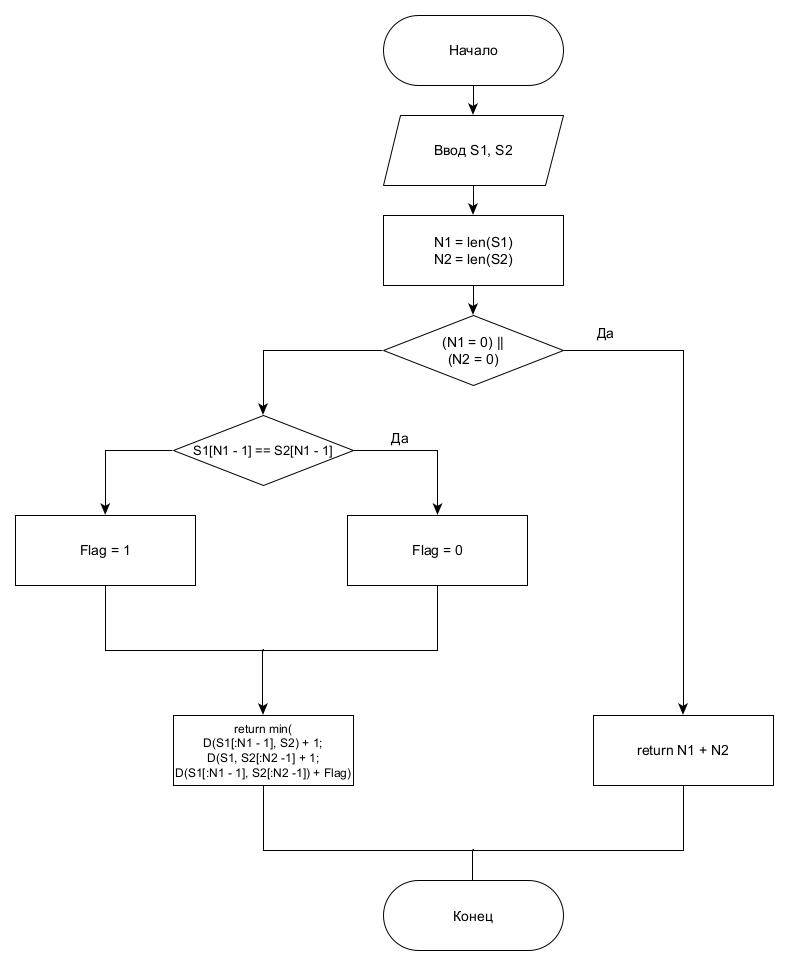
\includegraphics[width=\linewidth]{graph/LevenRec.jpg}
    \end{center}
    \caption{Схема рекурсивного алгоритма Левенштейна без матрицы}
\end{figure}

\begin{figure}[hp]
    \begin{center}
        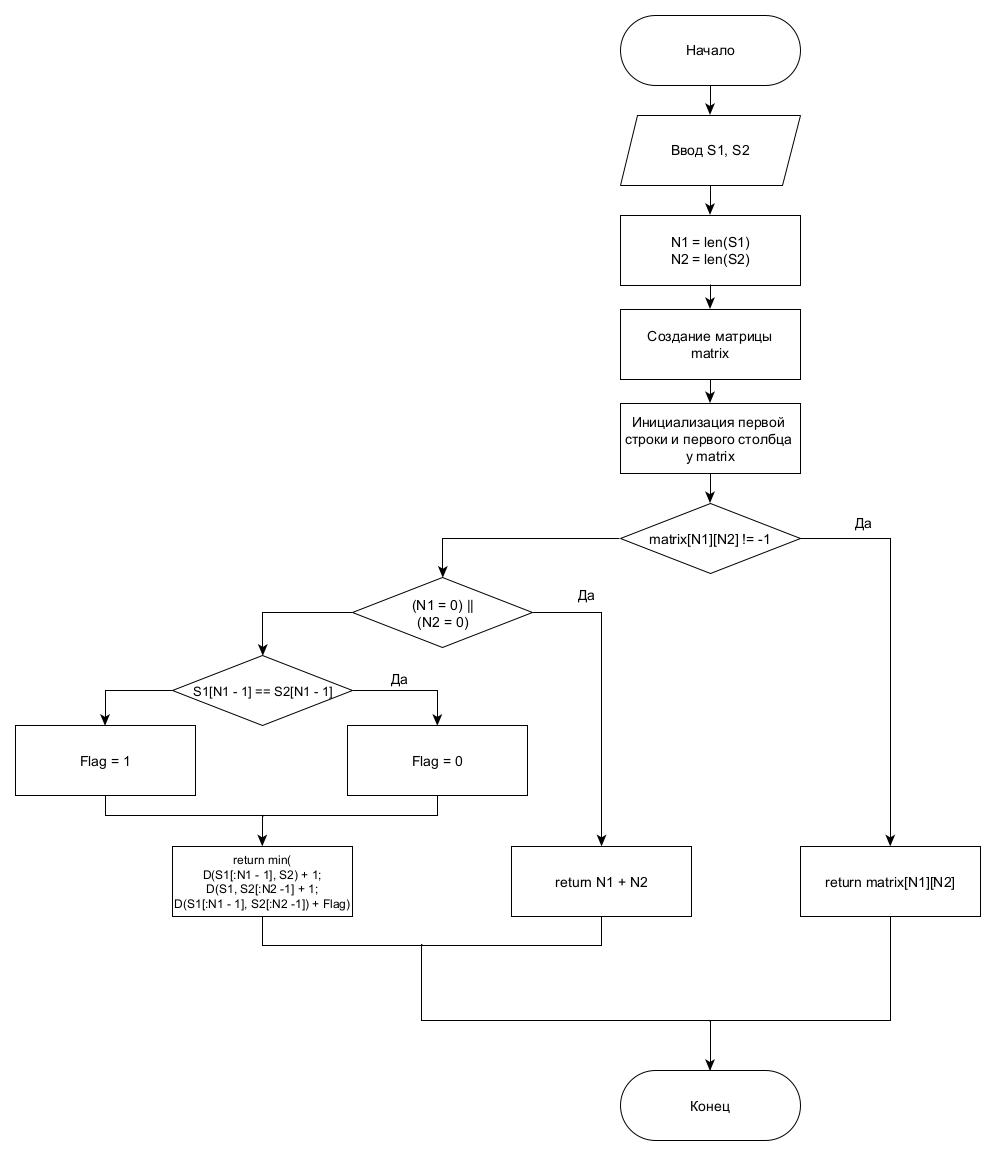
\includegraphics[width=\linewidth]{graph/LevenRecMatr.jpg}
    \end{center}
    \caption{Схема рекурсивного алгоритма Левенштейна с матрицей}
\end{figure}

\begin{figure}[hp]
    \begin{center}
        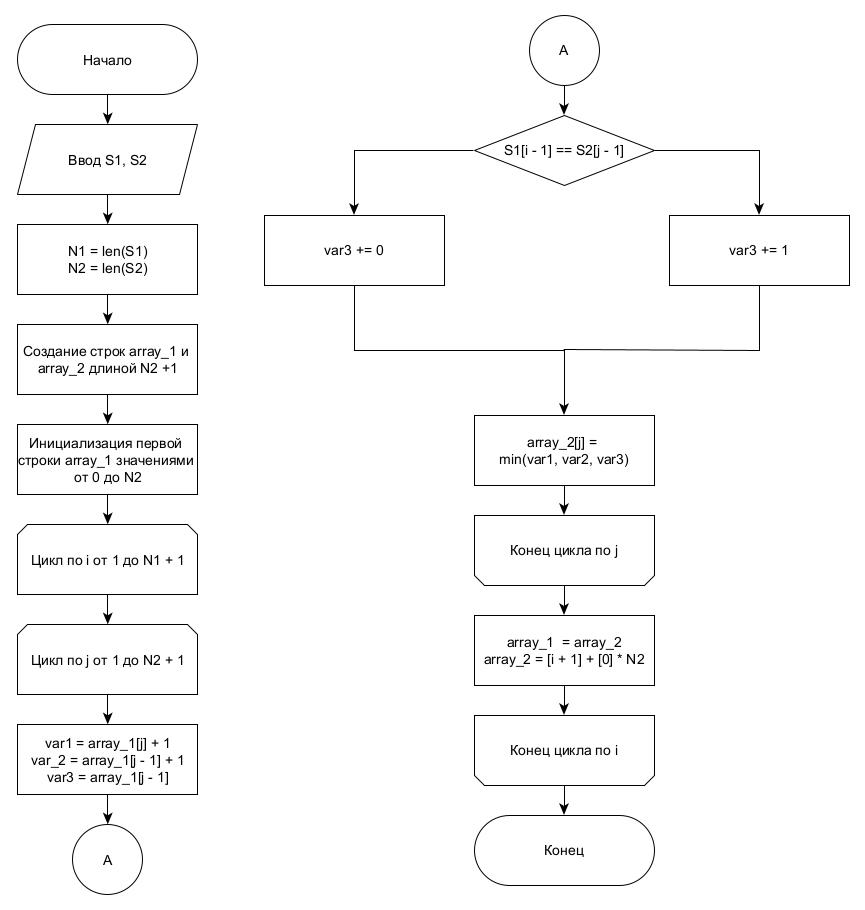
\includegraphics[width=\linewidth]{graph/LevenMatr.jpg}
    \end{center}
    \caption{Схема итеративного алгоритма Левенштейна с хранением двух строк}
\end{figure}
\begin{figure}[hp]
    \begin{center}
        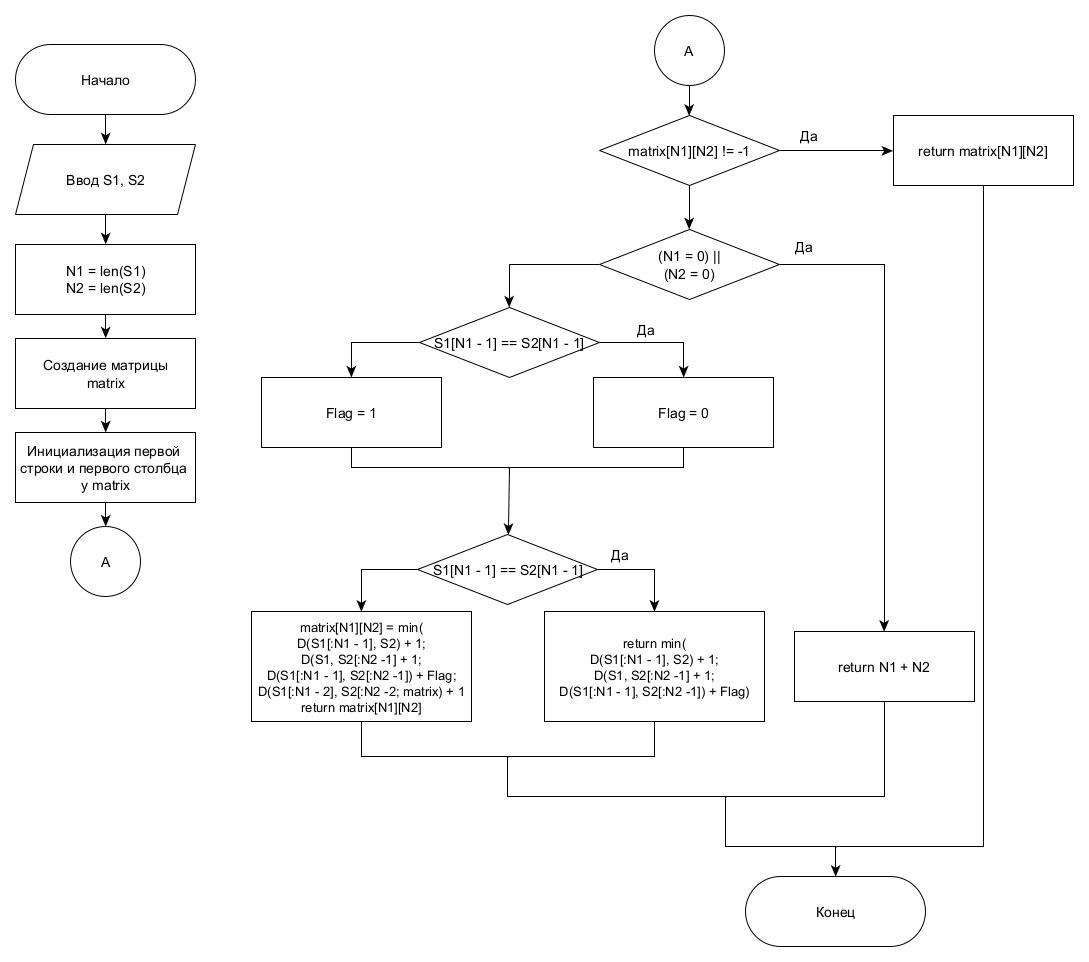
\includegraphics[width=\linewidth]{graph/Damerau.jpg}
    \end{center}
    \caption{Схема рекурсивного алгоритма Дамерау-Левенштейна (с матрицей)}
\end{figure}


\clearpage

\section{Вывод}
Были разработаны и протестированы спроектированные алгоритмы: вычисления расстояния Левенштейна рекурсивно, с заполнением матрицы и рекурсивно с заполнением матрицы, а также вычисления расстояния Дамерау — Левенштейна с заполнением матрицы.
